\section{ОБЗОР ЛИТЕРАТУРЫ}
\label{sec:domain}

%В обзоре литературы обычно содержится краткий анализ литературных источников различных типов,
%использованных в процессе работы над дипломным проектом.
%Здесь приводятся основные сведения, почерпнутые из литературы.
%Возможен анализ патентной чистоты.

\subsection{Python}
В современном мире скорость разработки программного обеспечения играет важную роль,
экономя не только время, но и средства, затраченные на разработку.
Таким свойством обладает один из высокоуровневых языков программирования — Python.
Помимо высокой скорости разработки Python также обладает следующими свойствами:
\begin{itemize}
    \item службы клиент/сервер, изображенные на рисунке~\ref{pic::domain::msg_types} как набор протоколов MMS;
    \item службы управления GOOSE/GSE;
    \item сервисы GSSE;
    \item сервисы синхронизации времени, изображенные на рисунке~\ref{pic::domain::msg_types} как SNTP.
\end{itemize}

Основными направлениями разработки на Python являются веб-приложения, Big Data, машинное обучение.

\subsection{Веб-приложение}
Веб-приложением принято называть программное обеспечение, предназначенное для выполнения определенных функций или задач через веб-браузер.
Веб-приложения отличаются от традиционных десктопных приложений тем, что не требуют установки на компьютер пользователя и могут быть запущены в любом совместимом веб-браузере.
Основными характеристиками веб-приложения являются:
\begin{itemize}
    \item Клиент-серверная архитектура:
    Веб-приложение включает в себя клиентскую часть (то, что видит и использует пользователь) и серверную часть (где хранятся данные и выполняются операции).
    Взаимодействие между клиентом и сервером происходит посредством
    ~\nomenclaturex{HTTP}{HyperText Transfer Protocol}{протокол передачи гипертекста} или
    ~\nomenclaturex{HTTPS}{HyperText Transfer Protocol Secure}{безопасный протокол передачи гипертекста}
    - протоколов прикладного уровня, седьмого уровня относительно модели~\nomenclaturex{OSI}{Open Systems Interconnection}{взаимосвязь открытых систем}.
    \item Доступность через интернет:
    Веб-приложения доступны для пользователей через интернет, что позволяет им использовать приложение из любой точки мира, где есть доступ к сети.
    \item Обновление и сопровождение:
    Одним из преимуществ веб-приложений является возможность централизованного обновления и сопровождения.
    Изменения в приложении могут быть внесены на сервере и автоматически доступны всем пользователям без необходимости обновления на стороне клиента.
\end{itemize}

\subsection{Веб-фреймворк}
Говоря простыми словами, фреймворк - это набор инструментов, ускоряющих разработку приложений.
Веб-фреймворк упрощает разработку и избавляет от необходимости написания рутинного кода при создании
динамических веб-сайтов, сетевых приложений, сервисов или ресурсов.
Для языка программирования Python существует несколько популярных веб-фреймворков:
\begin{itemize}
    \item Django
    \item \nomenclaturex{DRF}{Django Rest Framework}{веб-фреймворк на Python}
    \item Flask
    \item FastAPI
\end{itemize}

\subsection{Django и DRF}
Одним из популярных веб-фреймворком на Python является Django.
Он знаменит большим количеством функционала «из коробки», а именно:
\begin{itemize}
    \item Django~\nomenclaturex{ORM}{Object Related Mapper}{объектно-реляционное отображение}
    \item Django Admin Panel
    \item Защита от уязвимостей:
    Django включает в себя множество встроенных механизмов для обеспечения безопасности веб-приложений, таких как защита от
    CSRF-атак,
    SQL-инъекций,
    XSS-атак и многих других видов угроз.
\end{itemize}
стоит использовать DRF: Для быстрой разработки API.
Готовые компоненты: сериализаторы, представления, маршрутизация и система аутентификации – значительно упрощают создание API.
Это позволяет сосредоточиться на самой бизнес-логике, а не на написании основного кода с нуля.
\nomenclaturex{MVC}{Model View Controller}{модель, отображение, контроллер}

\subsection{ORM}
...

\subsection{\nomenclaturex{REST}{REpresentational State Transfer}{передача репрезентативного состояния}}
...

\subsection{FastAPI}
...

\subsection{PostgreSQL}
...

\subsection{MongoDB}
...

\subsection{Микросервисная архитектура}
...

\subsection{Брокеры сообщений}
...

\subsection{Apache Kafka}
...

\subsection{Docker}
...

%\subsection{Трейдинговая платформа}


%\nomenclaturex{OSI}{Open Systems Interconnection}{взаимосвязь открытых систем}
%Эталонная модель OSI детализирует модель, основанную на концепции многоуровневой
%коммуникационной функциональности. Модель конкретизирует семь уровней и выделяет
%функциональные требования для каждого уровня, чтобы создать надежную систему связи.
%Она не определяет протоколы, которые должны использоваться для достижения
%функциональности, и не ограничивает решение одним набором протоколов.
%
%\begin{figure}[ht]
%    \centering
%    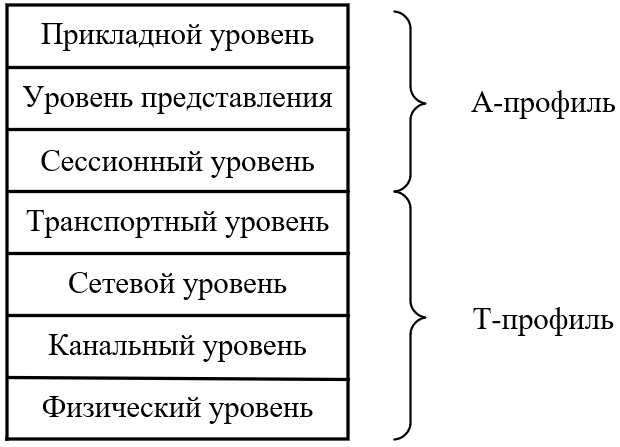
\includegraphics[width=.5\linewidth]{osiModel}
%    \caption{Эталонная модель и профили OSI}
%    \label{pic::domain::osi_model}
%\end{figure}
%
%В модели OSI используется два основных профиля: A-профиль -- профиль приложения
%и T-профиль -- транспортный профиль. Профили сопоставлены с уровнями модели,
%как изображено на рисунке~\ref{pic::domain::osi_model}. А-профиль OSI --
%это набор спецификаций и соглашений, которые относятся к трем верхним уровням
%эталонной модели OSI (уровень приложения, уровень представления и сессионный
%уровень). Т-профиль относится к четырем нижним уровням модели
%(транспортный уровень, сетевой, канальный и физический). Можно использовать
%различные комбинации А- и Т-профилей, чтобы обеспечить определенные виды информации
%и сервисов, подлежащих обмену. Сервисы представлены в четырех различных комбинациях
%А- и Т-профилей. Они используются для следующих служб:
%
%\begin{itemize}
%    \item службы клиент/сервер, изображенные на рисунке~\ref{pic::domain::msg_types} как набор протоколов MMS;
%    \item службы управления GOOSE/GSE;
%    \item сервисы GSSE;
%    \item сервисы синхронизации времени, изображенные на рисунке~\ref{pic::domain::msg_types} как SNTP.
%\end{itemize}
%
%\nomenclaturex{GSSE}{Generic Substation State Event}{обобщенное событие состояния подстанции}
%\nomenclaturex{GSE}{Generic Substation Event}{обобщенное событие подстанции}

% \subsection{Существующие аналоги}

% TODO: implement
